%%%%%%%%%%%%%%%%%%%%%%%%%%%%%%%%%%%%%%%%%
% Fancyslides Presentation
% LaTeX Template
% Version 1.0 (30/6/13)
%
% This template has been downloaded from:
% http://www.LaTeXTemplates.com
%
% The Fancyslides class was created by:
% Paweł Łupkowski (pawel.lupkowski@gmail.com)
%
% License:
% CC BY-NC-SA 3.0 (http://creativecommons.org/licenses/by-nc-sa/3.0/)
%
%%%%%%%%%%%%%%%%%%%%%%%%%%%%%%%%%%%%%%%%%

%----------------------------------------------------------------------------------------
%	PACKAGES AND OTHER DOCUMENT CONFIGURATIONS
%----------------------------------------------------------------------------------------

\documentclass{fancyslides}

\usepackage[utf8]{inputenc} % Allows the usage of non-english characters
\usepackage{times} % Use the Times font
\usepackage{booktabs} % Allows the use of \toprule, \midrule and \bottomrule in tables
\graphicspath{{images/}} % Location of the slide background and figure files

% Beamer options - do not change
\usetheme{default} 
\setbeamertemplate{navigation symbols}{} % Disable the slide navigation buttons on the bottom of each slide
\setbeamercolor{structure}{fg=\yourowntexcol} % Define the color of titles and fixed text elements (e.g. bullet points)
\setbeamercolor{normal text}{fg=\yourowntexcol} % Define the color of text in the presentation

%------------------------------------------------
% COLORS
% The following colors are predefined in this class: white, black, gray, blue, green and orange

% Define your own color as follows:
\definecolor{bulgarianrose}{rgb}{0.28,0.02,0.03}
\definecolor{rose}{rgb}{0.54,0.2,0.14}
\definecolor{charcoal}{rgb}{.021,0.27,0.31}
\newcommand{\structureopacity}{0.75} % Opacity (transparency) for the structure elements (boxes and circles)

\newcommand{\strcolor}{charcoal} % Set the color of structure elements (boxes and circles)
\newcommand{\yourowntexcol}{white} % Set the text color

%----------------------------------------------------------------------------------------
%	TITLE SLIDE
%----------------------------------------------------------------------------------------

\newcommand{\titlephrase}{Spatially Random Processes in
  One-Dimensional Maps: The Logistic Map and The Arnold Circle Map} % Presentation title
\newcommand{\name}{Amy Le} % Presenter's name
\newcommand{\affil}{CU Boulder} % Presenter's institution
\newcommand{\email}{April 16, 2015} % Presenter's email address

\begin{document}

\startingslide % This command inserts the title slide as the first slide

%----------------------------------------------------------------------------------------
%	PRESENTATION SLIDES
%----------------------------------------------------------------------------------------

%\fbckg{1.jpg} % Slide background image
\begin{frame}
\itemized{
\item Groundwater Contamination
\item Spatially Random Processes
\item Implementation in the Logistic Map and the Circle Map
}
%\pointedsl{} % Text in this environment is printed in a circle and will be made large and uppercase - if you need to fit more text in you can reduce the font size within the \pointedsl{} bracket as usual, e.g. \pointedsl{\large smaller main point}
\end{frame}
%------------------------------------------------

\begin{frame}
\misc{ % Anything can be placed inside the \misc{} command
The total groundwater withdrawls in the United States in 2005, categorized
  in terms of use.
\begin{figure}[h]
\centering
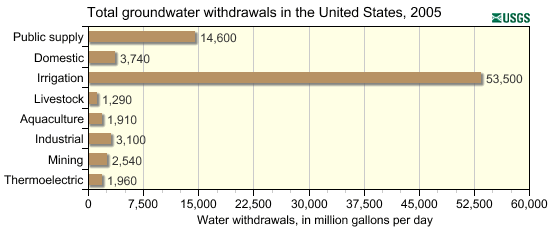
\includegraphics[scale=0.7]{gwuse}
\end{figure}
}
\end{frame}
%------------------------------------------------
\fbckg{Sources-of-Contamination}
\begin{frame}
\end{frame}
%------------------------------------------------
\fbckg{blank}
\begin{frame}
\misc{ % Anything can be placed inside the \misc{} command
Typical porosity and hydraulic conductivity ranges for clay, sand, and gravel.
\begin {table}[h]
\begin{center}
    \begin{tabular}{ l l l l}
    \toprule
    Grain Size & Material & Porosity & Hydraulic Conductivity $K$
    (m/s)\\ 
\midrule
    Fine & Clay  &  50\% &$[5\times 10^{-9}, 5\times 10^{-6}]$\\ 
    Medium &  Sand & 25\% & $[10^{-8},10^{-6}]$\\ 
    Coarse &  Gravel &  20\% & $[5 \times 10^{-4}, 5 \times 10^{-2}]$\\ 
    \end{tabular}
\end{center}
\end{table}
}
\end{frame}
%------------------------------------------------
\begin{frame}
\misc{ 
\begin{figure}[h]
\centering
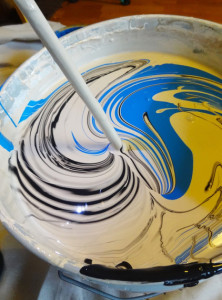
\includegraphics[scale=0.65]{Mixing-Paint-222x300}
\end{figure}
}
\end{frame}
%------------------------------------------------
\begin{frame}
\itemized{
\item Transmissivity as a random function of space
\item 3-D model with incompressible fluid $\to$ Fluid flow as
  a 1-D map
\item Injecting treatment solution in the aquifer $\leftrightarrow$ initial condition
}
\end{frame}

%------------------------------------------------
\begin{frame}
\pointedsl{\large Spatially Random Processes} % Text in this environment is printed in a circle and will be made large and uppercase - if you need to fit more text in you can reduce the font size within the \pointedsl{} bracket as usual, e.g. \pointedsl{\large smaller main point}
\end{frame}

%------------------------------------------------
\begin{frame}
%\framedsl{} 
\misc{Log-normal noise 
\begin{align*}
\begin{split}
R(x) &= e^{\xi(x)}\\
%\xi(x)&=\ln(R(x)) \\
\mu&=E[\xi(x)]=\ln(r) \>, \quad \sigma^2 = Var(\xi(x))\\
\xi(x)&= \ln(r) + \sum_{n \in \mathbb{Z}}\hat{\xi}_ne^{2\pi inx}\>, \quad  \hat{\xi}_n \in \mathbb{C}\\
%\hat{\xi}_{n}^* &= \hat{\xi}_{-n} \>, \quad  \hat{\xi}_n \in \mathbb{C}\\
\hat{\mu}_n&=E[\hat{\xi}_n]=0\>, \quad \hat{\sigma}_n^2=\alpha e^{-L|n|}
\end{split}
\end{align*}
}
\end{frame}
%------------------------------------------------
% \begin{frame}
% \misc{ 
% \begin{itemize}
% \item The correlation function $C(x)$
% \item The spectral density $S(n)$
% \end{itemize}
% $L=0.5,\sigma=0.0216, \alpha=0.000114$
% \begin{figure}[h]
% \centering
% 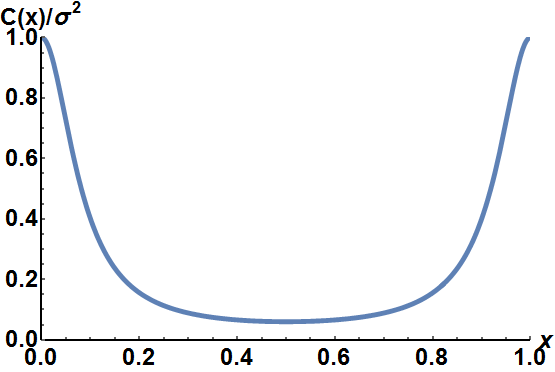
\includegraphics[width=.48\textwidth]{cx}\hfill
% 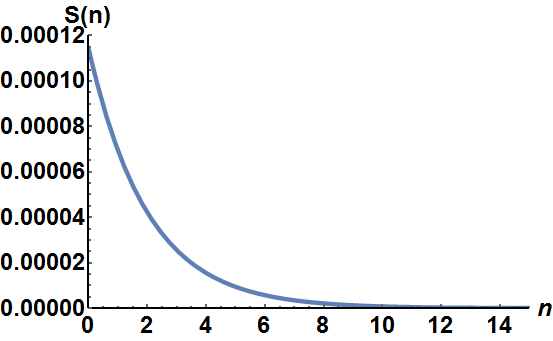
\includegraphics[width=.51\textwidth]{sn}
% \end{figure}
% }
% \end{frame}
%------------------------------------------------
% \begin{frame}
% \misc{
% Spectral density, variance of $\hat{\xi}_n$, and covariance of $\xi(x)$
% \begin{align*}
% \begin{split}
% \hat{\sigma}_n^2&=S(n)\\
% S(n)&=\alpha e^{-L|n|}\>, \quad  L \in (0,\infty), \alpha \in \mathbb{R}\\
% C(x) &= \sum_{n\in \mathbb{Z}}S(n)e^{2\pi inx}
% \end{split}
% \end{align*}
% }
% \end{frame}

%------------------------------------------------

% \begin{frame}
% \misc{ % Anything can be placed inside the \misc{} command
% The function $R:[0,1]\to [0,4]$ where $\hat{\xi}_n \sim
% Unif(-M_n,M_n), \sigma=0.0386, L=0.1, r=3.5, N=100$
% \begin{figure}[h]
% \centering
% 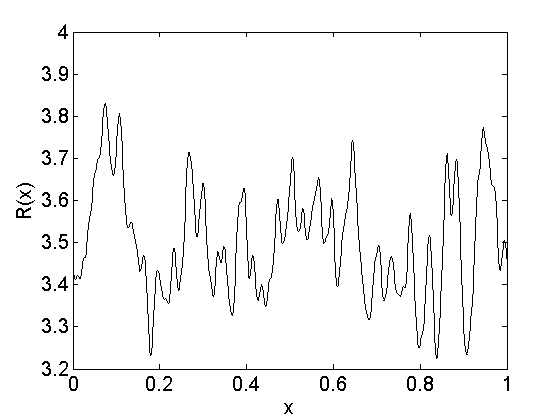
\includegraphics[scale=0.5]{xi}
% \end{figure}
% }
% \end{frame}
%------------------------------------------------

% \begin{frame}
% \misc{ 
% The function $\Omega:\mathbb{R}^+ \to \mathbb{R}^+$ where $\hat{\xi}_n \sim
% N(0,\hat{\sigma}_n^2), L=0.1, r=0.7, \alpha = 10^{-6}, N=100$
% \begin{figure}[h]
% \centering
% 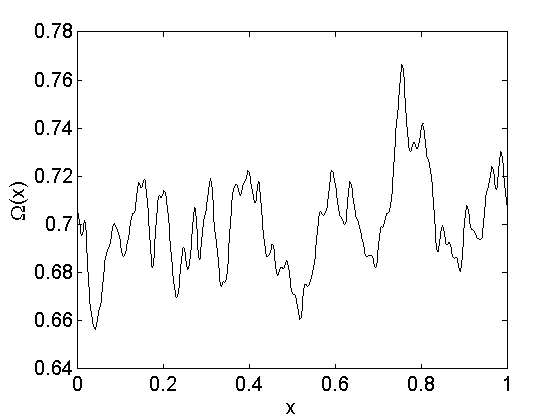
\includegraphics[scale=0.5]{Omega}
% \end{figure}
% }
% \end{frame}
%------------------------------------------------
\begin{frame}
\pointedsl{\large One-Dimensional Maps} 
 \end{frame}

%------------------------------------------------
\begin{frame}
\misc{ 
Chaos is aperiodic long-term behavior in a deterministic
  system that exhibits sensitive dependence on initial conditions.
}
 \end{frame}
%------------------------------------------------
\begin{frame}
\misc{ Fixed Point Iteration
\begin{align*}
\begin{split}
f(x^*) &= x^*\\
0&=f(x^*)-x^*
\end{split}
\end{align*}
}
 \end{frame}

%------------------------------------------------
\fbckg{blank}
\begin{frame}
\framedsl{Logistic Map} 
\misc{
\begin{align*}
\begin{split}
x_{n+1} &=  rx_n(1-x_n)\>, \quad  r \in [0,4]\\
x_{n+1}= f_l(x_n) &=  R(x_n)x_n(1-x_n)\>, \quad  R(x_n) \in [0,4]\\
\end{split}
\end{align*}
}
\end{frame}
%------------------------------------------------
\fbckg{blank}
\begin{frame}
\framedsl{\large Spatially Random Process} 
\misc{
\begin{align*}
\begin{split}
\xi(x)&= \ln(r) + \sum_{n \in \mathbb{Z}}\hat{\xi}_ne^{2\pi inx}\\
\sigma &\in \left[0,\ln\left(\frac{4}{r}\right)\sqrt{\frac{2}{3}}\frac{\tanh(L/4)}{\sqrt{\tanh(L/2)}}\right]
\end{split}
\end{align*}
}
\end{frame}
%------------------------------------------------
% \begin{frame}
% \misc{ Cobweb Diagrams\\
% $x_{n+1}=f(x_n)$
% \begin{figure}[h]
% \centering
% 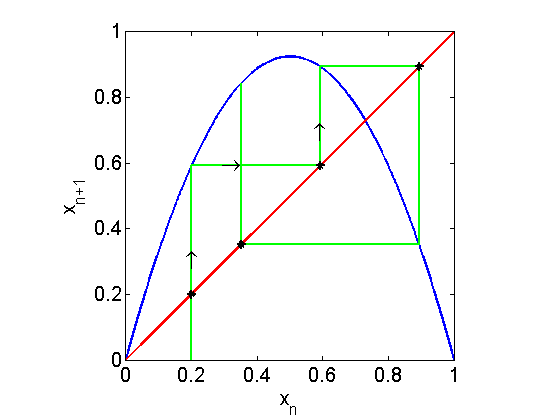
\includegraphics[scale=0.5]{cobweb_ex}
% \end{figure}
% }
% \end{frame}

%------------------------------------------------
\begin{frame}
\misc{ Orbit Diagrams\\
\begin{itemize}
\item Deterministic logistic map, $r=3.2$
\item A random realization, $r=3.2,\sigma=0.0204$ 
\end{itemize}
\begin{figure}[h]
\centering
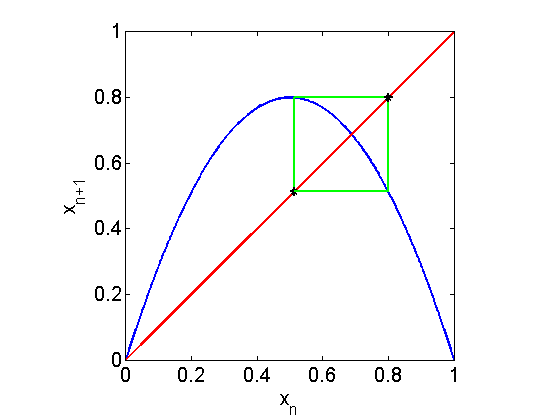
\includegraphics[width=.495\textwidth]{det_cobweb}\hfill
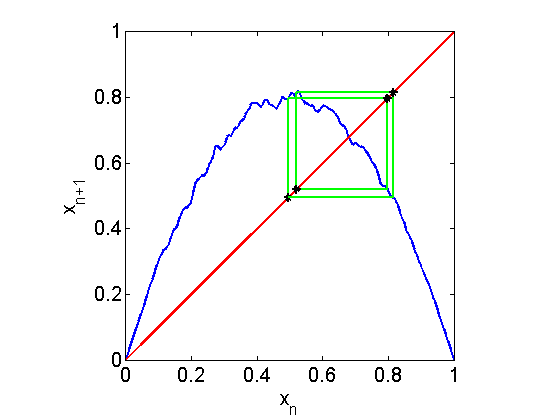
\includegraphics[width=.495\textwidth]{rand_cobweb}
\end{figure}
}
\end{frame}
%------------------------------------------------

\fbckg{blank}
\begin{frame}
\framedsl{Circle Map} 
\misc{
\begin{align*}
\begin{split}
x_{n+1} &= x_n + \omega - \frac{k}{2\pi}\sin(2\pi x_n)\>, \quad  \omega \>, k \in \mathbb{R}  \\
x_{n+1}= f_c(x_n) &=  x_n + \Omega(x_n) - \frac{k}{2\pi}\sin(2\pi x_n)\>, \quad  \Omega(x_n)\>, k \in \mathbb{R}  
\end{split}
\end{align*}
}
\end{frame}
%------------------------------------------------
\fbckg{blank}
\begin{frame}
\framedsl{\large Spatially Random Process} 
\misc{
\begin{align*}
\begin{split}
\xi(x)&= \ln(\omega) + \sum_{n \in \mathbb{Z}}\hat{\xi}_ne^{2\pi inx}\\
\hat{\sigma}_n^2 &= \alpha e^{-L|n|}
\end{split}
\end{align*}
}
\end{frame}

%------------------------------------------------
\begin{frame}
\misc{ Orbit Diagrams\\
\begin{itemize}
\item Deterministic circle map, $k=1,\omega=0.3$
\item A random realization, $k=1,\omega=0.3,\alpha = 10^{-5}$
%$\hat{\xi}_n \sim N(0,\hat{\sigma}_n^2),\alpha = 10^{-5},L=0.1, N=100$
\end{itemize}
\begin{figure}[h]
\centering
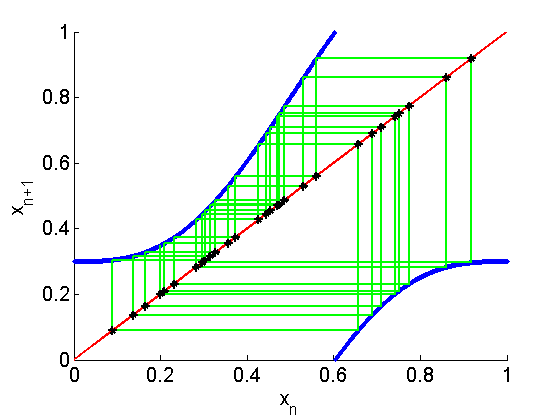
\includegraphics[width=.495\textwidth]{detcirc_cobweb}\hfill
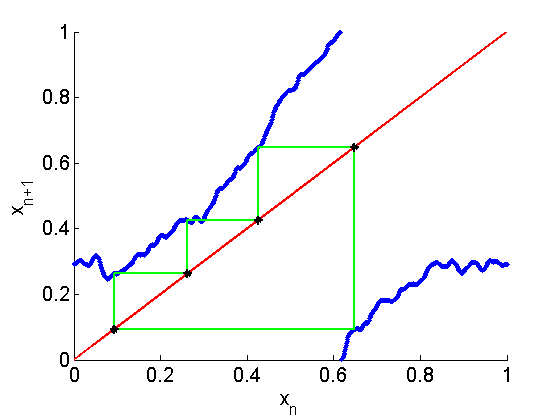
\includegraphics[width=.495\textwidth]{randcirc_norm_cobweb}\hfill
\end{figure}
}
\end{frame}

% %------------------------------------------------
% \begin{frame}
% \pointedsl{\small Distributions of Random Variables} 
%  \end{frame}

% %------------------------------------------------

% \begin{frame}
% \misc{
% Choosing a distribution: uniform 
% \begin{align*}
% \begin{split}
% \hat{\xi}_n &\sim Unif(-M_n,M_n)
% \end{split}
% \end{align*}
% \begin{equation*}
%    h_u(a_n,b_n)= \left\{
%      \begin{array}{lr}
%        \frac{1}{4 M_n^2} & |a_n|,|b_n| \leq M_n\\
%        0 & |a_n|,|b_n| > M_n\\
%      \end{array}
%    \right.
% \end{equation*} 
% }
% \end{frame}

% %------------------------------------------------
% \begin{frame}
% \misc{
% Choosing a distribution: Gaussian 
% \begin{equation*}
% \hat{\xi}_n \sim N(0,\hat{\sigma}_n^2)
% \end{equation*}
% \begin{equation*}
%    h_g(x) = \frac{1}{\hat{\sigma}_n \sqrt{2\pi}}e^{-\frac{x^2}{2\hat{\sigma}_n^2}}
% \end{equation*} 
% }
% \end{frame}
%------------------------------------------------
\fbckg{blank}
\begin{frame}
\pointedsl{\large Bifurcations} 
 \end{frame}

%------------------------------------------------
\fbckg{blank}
\begin{frame}
\misc{Bifurcation Diagram: Logistic Map
\begin{figure}[h]
\centering
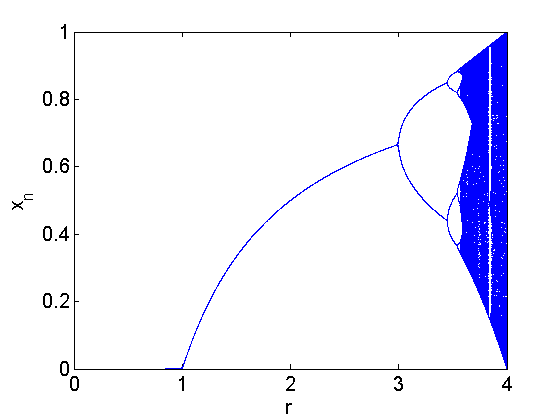
\includegraphics[width=.495\textwidth]{det_bif_1}\hfill
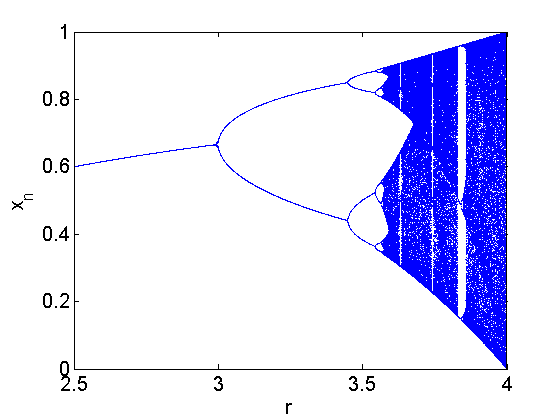
\includegraphics[width=.495\textwidth]{det_bif_2}
\end{figure}
}
\end{frame}
%------------------------------------------------
\fbckg{rlog_bif_L_01} 
\begin{frame}
\end{frame}
%------------------------------------------------
\fbckg{rlog_bif_L_09} 
\begin{frame}
\end{frame}
%------------------------------------------------
\fbckg{rlog_bif_halfs_L_01} 
\begin{frame}
\end{frame}
%------------------------------------------------
\fbckg{rlog_bif_halfs_L_09} 
\begin{frame}
\end{frame}
%------------------------------------------------
\fbckg{blank}
\begin{frame}
\pointedsl{\large Lyapunov Exponents} 
 \end{frame}
%------------------------------------------------
\fbckg{blank}
\begin{frame}
\misc{ The Lyapunov Exponent
\begin{itemize}
\item The deterministic map
\item Randomized system over $N_\lambda  =10,000$ simulations, $L=0.1$
\end{itemize}
\begin{figure}[h]
\centering
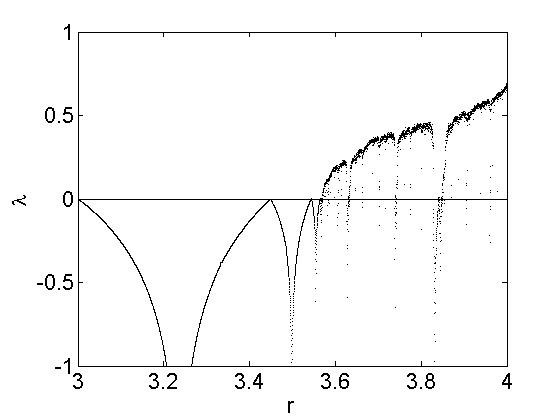
\includegraphics[width=.495\textwidth]{det_log_lyap}\hfill
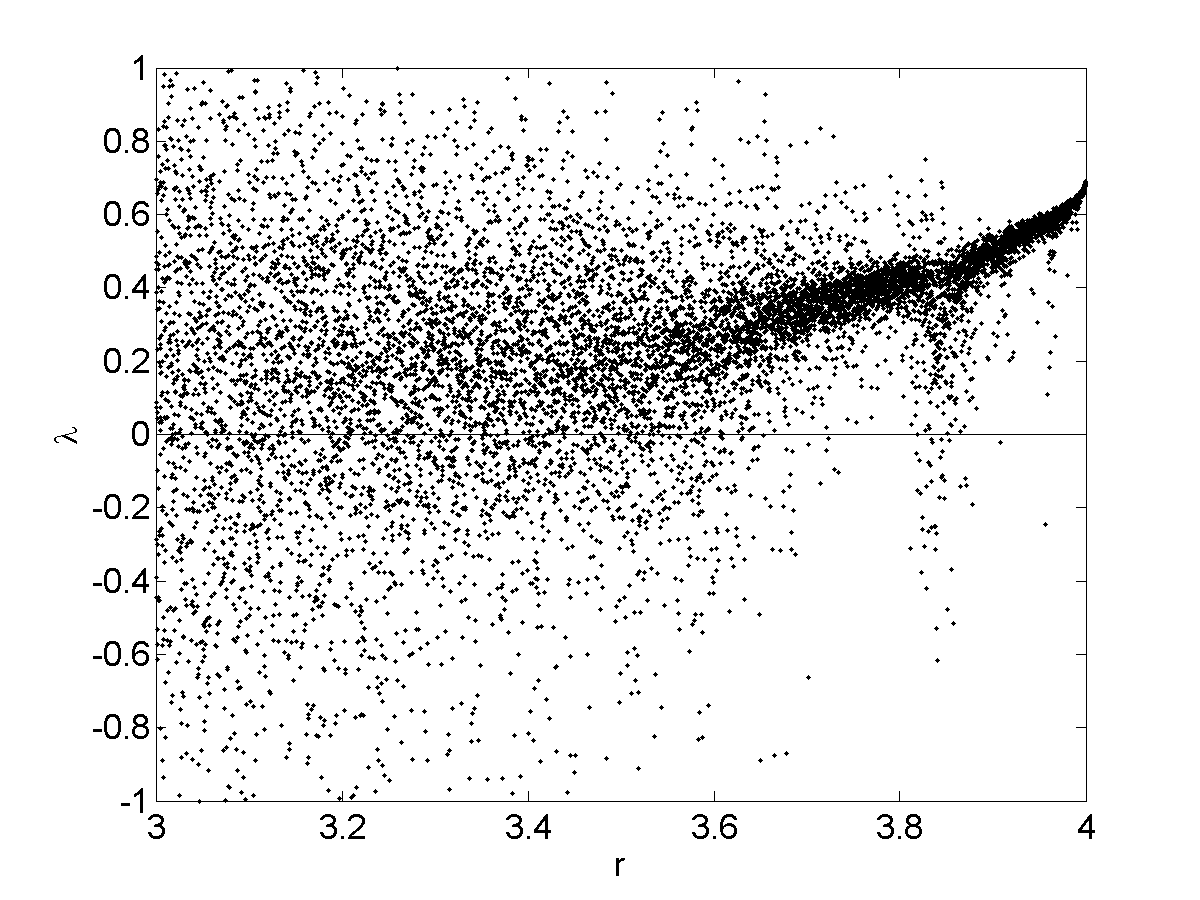
\includegraphics[width=.495\textwidth]{rlog_lyap_L_01}
\end{figure}
}
\end{frame}
%------------------------------------------------
% \fbckg{blank} % Slide background image
% \begin{frame}
% \misc{\pitem{Randomness has stabilizing effect on the logistic map}
%   \pitem{Preservation of some features of Lyapunov exponents}
%   \fitem{Noise is not log-normal}} 
% \end{frame}
\fbckg{blank}
\begin{frame}
\pointedsl{\large Period Distribution} 
 \end{frame}
%------------------------------------------------
\fbckg{rlog_hist_L_01_r_33_s_0017565_a_15414e-05_sims_5000}
\begin{frame}
 \end{frame}
%------------------------------------------------
\fbckg{rlog_hist_L_09_r_33_s_005351_a_0001208_sims_5000}
\begin{frame}
 \end{frame}
%------------------------------------------------
\fbckg{blank}
\begin{frame}
\misc{ The Arnold Tongues of the Circle Map\\
%$\omega \in [0,1], \Delta \omega = 0.001, k \in [0,1.5],\Delta k = 0.0015, p_{max}=100$
\begin{figure}[h]
\centering
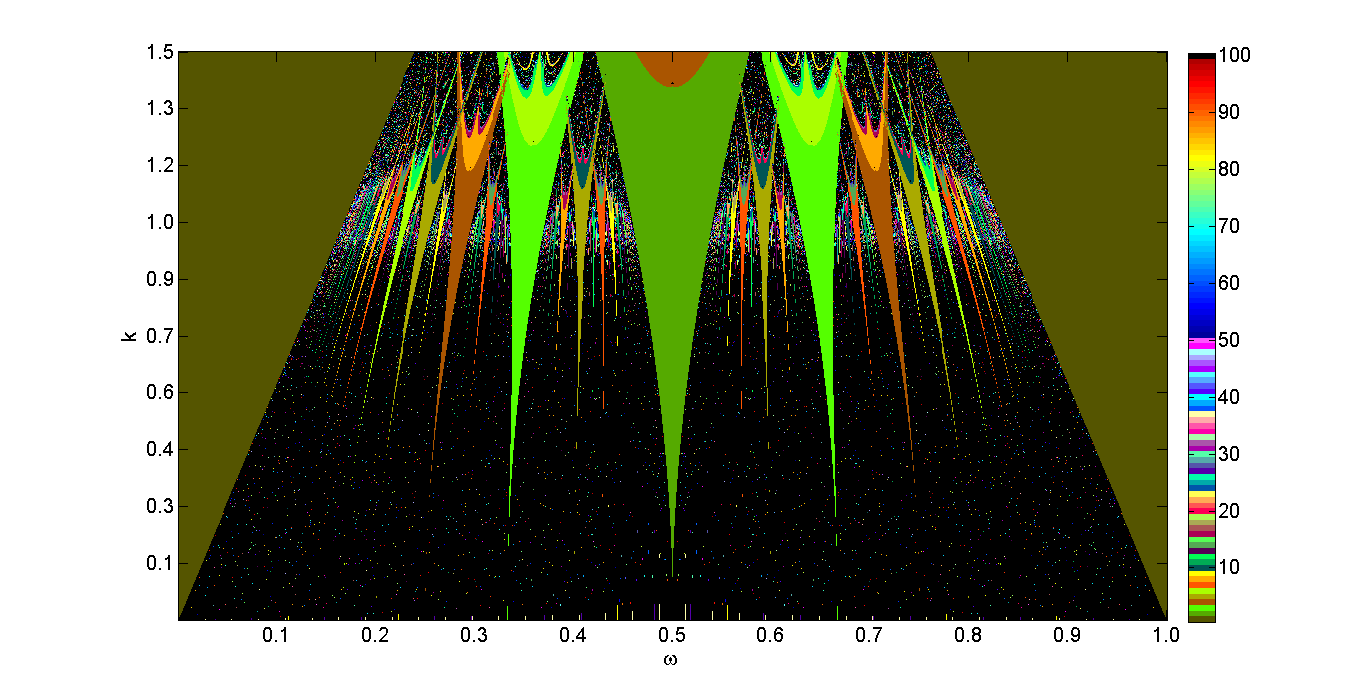
\includegraphics[scale=0.28]{tongues_1000_det}
\end{figure}
}
\end{frame}
%------------------------------------------------
\fbckg{tongues_norm_1000_L_01} 
\begin{frame}
\end{frame}
%------------------------------------------------
\fbckg{tongues_norm_1000_L_03} 
\begin{frame}
\end{frame}
%------------------------------------------------
\fbckg{tongues_norm_1000_L_05} 
\begin{frame}
\end{frame}
%------------------------------------------------
\fbckg{blank}
\begin{frame}
\misc{ The Lyapunov Exponent of the Circle Map\\
$N_\lambda = 10,000$ simulations, $\alpha = 10^{-5}$, $L=0.1$
\begin{figure}[h]
\centering
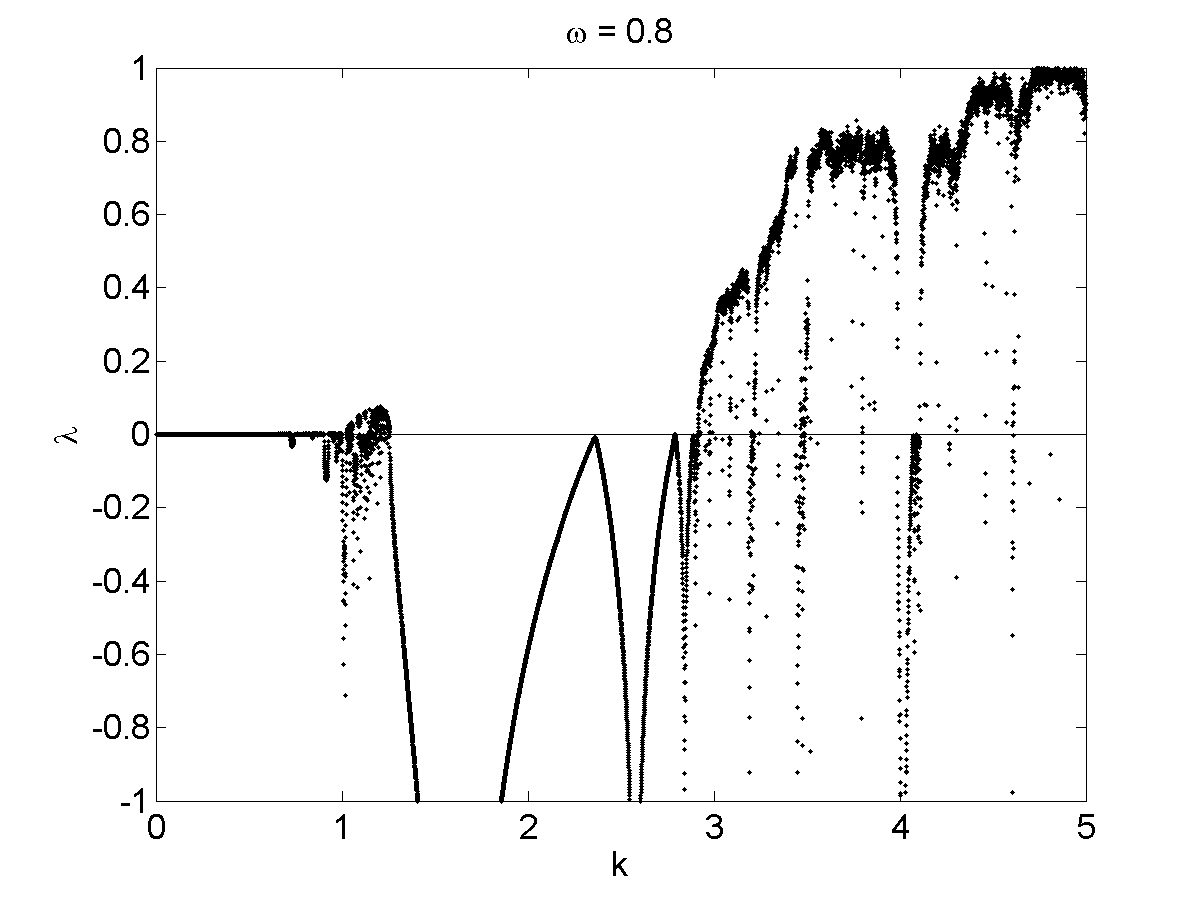
\includegraphics[width=.495\textwidth]{detcirc_n_lyap_10000_w_08_k}\hfill
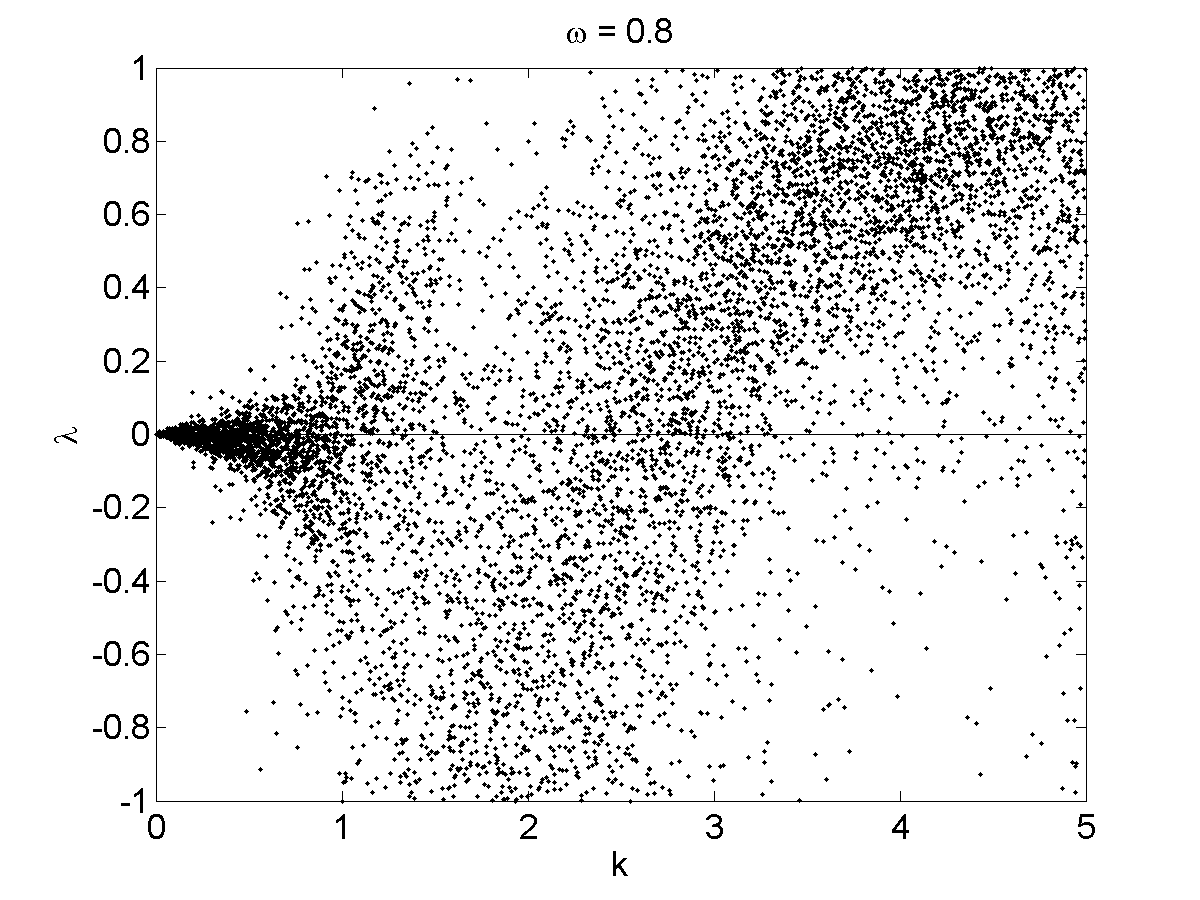
\includegraphics[width=.495\textwidth]{rcirc_n_lyap_10000_L_01_w_08_k}
\end{figure}
}
\end{frame}
%------------------------------------------------
\fbckg{blank}
\begin{frame}
\misc{ The Lyapunov Exponent of the Circle Map\\
$N_\lambda = 10,000$ simulations, $\alpha = 10^{-5}$, $L=0.1$
\begin{figure}[h]
\centering
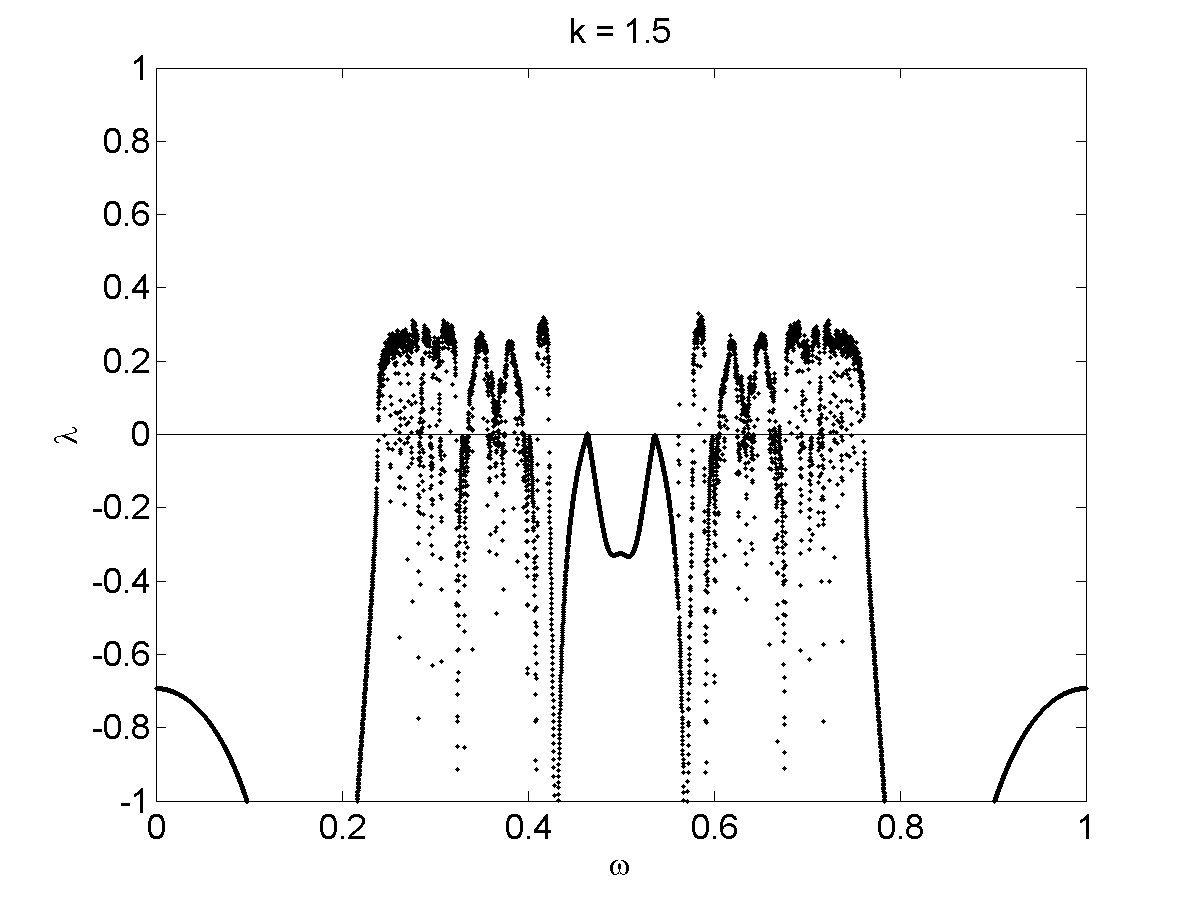
\includegraphics[width=.495\textwidth]{detcirc_lyap_10000_k_15_w}\hfill
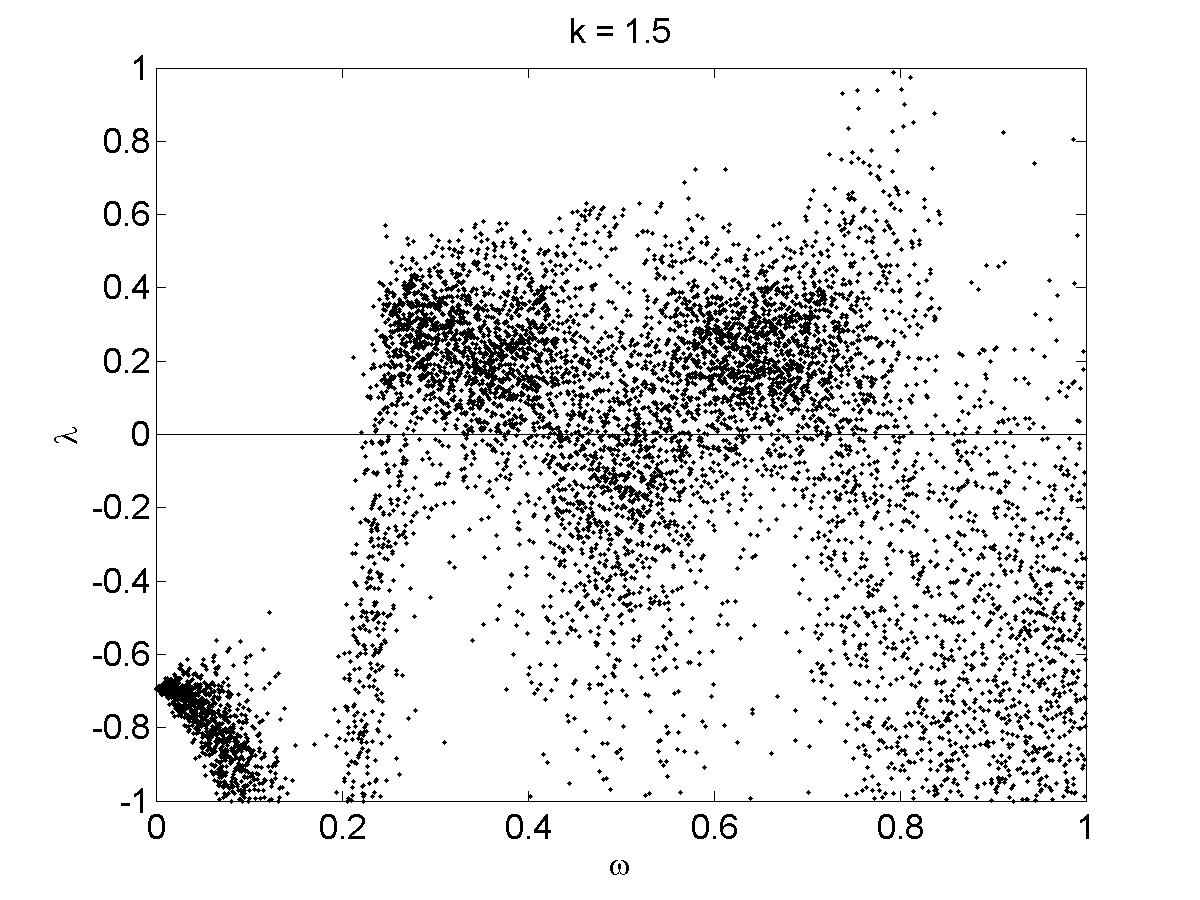
\includegraphics[width=.495\textwidth]{rcirc_n_lyap_L_01_w}
\end{figure}
}
\end{frame}
%------------------------------------------------
\fbckg{blank}
\begin{frame}
\misc{ Period Distribution
\begin{figure}[h]
\centering
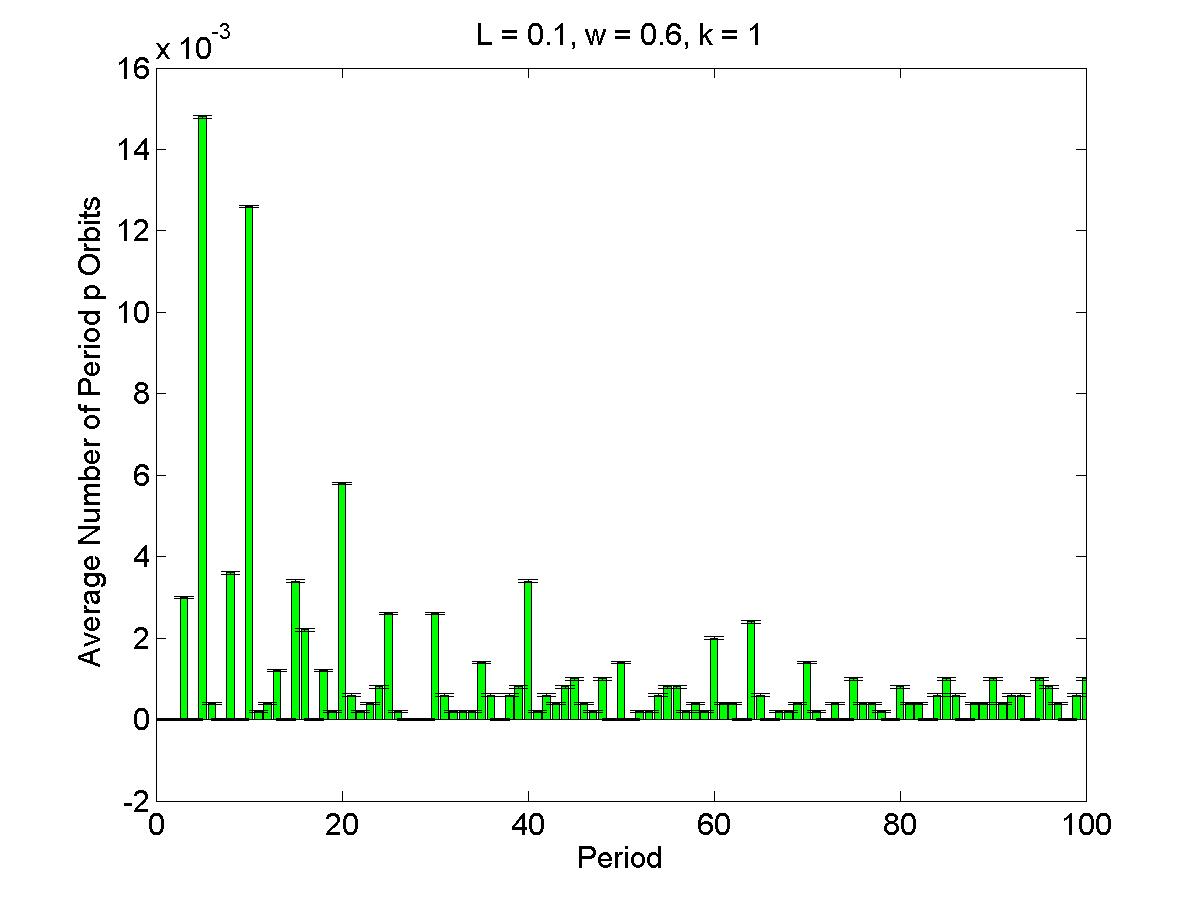
\includegraphics[width=.495\textwidth]{rcirc_hist_u_L_01_w_06_k_1_sims_5000}\hfill
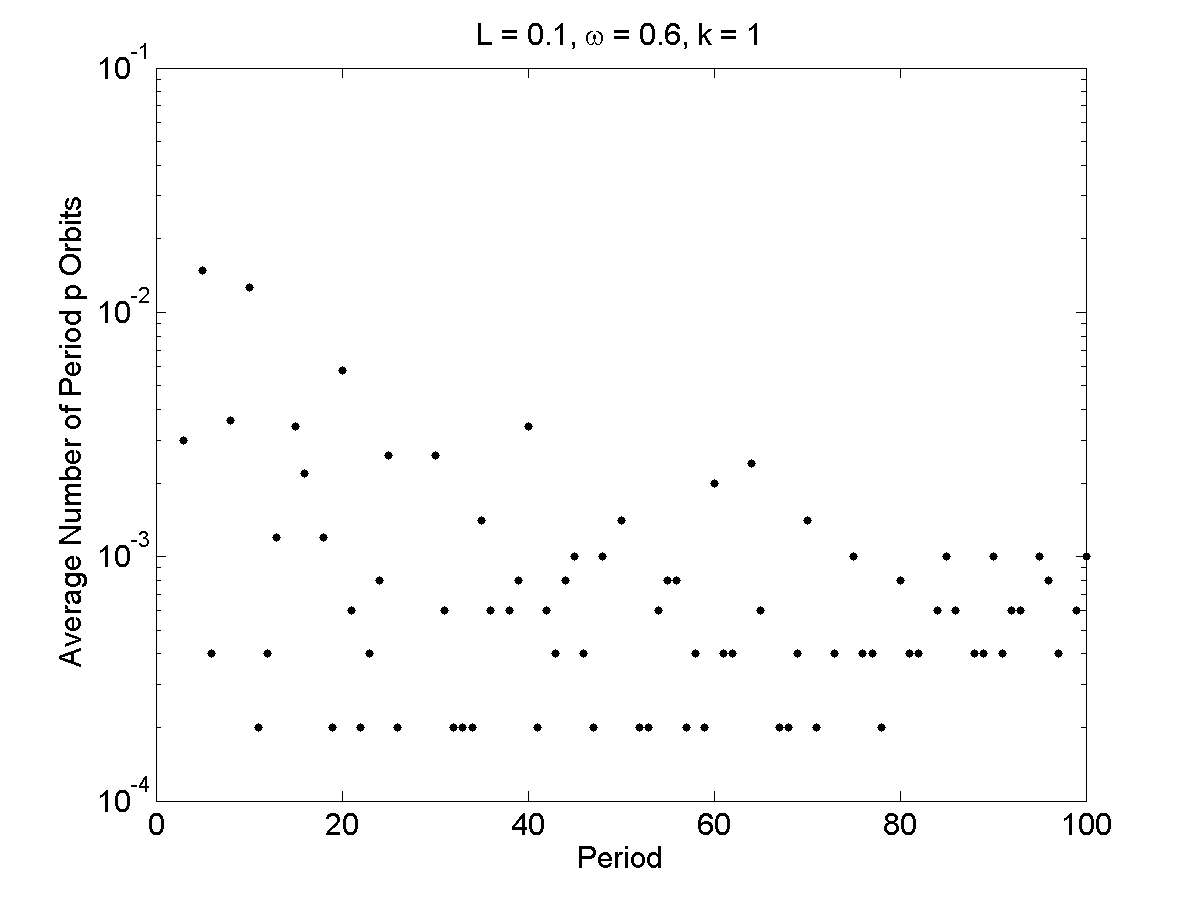
\includegraphics[width=.495\textwidth]{rcirc_avg_num_1000_sim_logscale}
\end{figure}
}
\end{frame}
%------------------------------------------------
\fbckg{blank}
\begin{frame}
\pointedsl{Conclusion} 
 \end{frame}
%------------------------------------------------
\fbckg{blank} % Slide background image
\begin{frame}
\misc{Logistic Map\\
\pitem{Stabilized low period region of logistic map for $r \in [3,4]$}
\pitem{High-period orbits for small $r$ present when $\sigma \approx \sigma_{max}$}
\fitem{Distribution of period may be exponential}} 
\end{frame}
%------------------------------------------------
\fbckg{blank} % Slide background image
\begin{frame}
\misc{Circle Map\\
\pitem{New period 2 region in the circle map for $L=0.3$}
\pitem{Asymmetry in tongues and Lyapunov exponents for small $L$}
\fitem{Distribution of period may not be exponential}} 
\end{frame}
%------------------------------------------------
\fbckg{blank}
\begin{frame}
\pointedsl{Future Work} 
 \end{frame}

%------------------------------------------------

\begin{frame}
\misc{\pitem{Lotka-Volterra system of ODEs or H\'{e}non map}
\pitem{Basin of attraction of chaotic trajectories}
\fitem{Distribution of zeroes of $\mathcal{F}(x)=f(x)-x$}} 
\end{frame}
%------------------------------------------------

\begin{frame}
\thankyou % Inserts a thank you slide
\end{frame}

%------------------------------------------------
\end{document}